\documentclass[a4paper,norsk, 10pt]{article}
\usepackage[utf8]{inputenc}
\usepackage{verbatim}
\usepackage{listings}
\usepackage{graphicx}
\usepackage[norsk]{babel}
\usepackage{a4wide}
\usepackage{color}
\usepackage{amsmath}
\usepackage{float}
\usepackage{amssymb}
\usepackage[dvips]{epsfig}
\usepackage[toc,page]{appendix}
\usepackage[T1]{fontenc}
\usepackage{cite} % [2,3,4] --> [2--4]
\usepackage{shadow}
\usepackage{hyperref}
\usepackage{titling}
\usepackage{marvosym }
\usepackage{subcaption}
\usepackage[noabbrev]{cleveref}
\usepackage{cite}


\setlength{\droptitle}{-10em}   % This is your set screw

\setcounter{tocdepth}{2}

\lstset{language=c++}
\lstset{alsolanguage=[90]Fortran}
\lstset{alsolanguage=Python}
\lstset{basicstyle=\small}
\lstset{backgroundcolor=\color{white}}
\lstset{frame=single}
\lstset{stringstyle=\ttfamily}
\lstset{keywordstyle=\color{red}\bfseries}
\lstset{commentstyle=\itshape\color{blue}}
\lstset{showspaces=false}
\lstset{showstringspaces=false}
\lstset{showtabs=false}
\lstset{breaklines}
\title{FYS2160 Oblig 1}
\author{Daniel Heinesen, daniehei}
\begin{document}
\maketitle


\section{Part 1)}
\subsection{a)}
For this system with $ N = 3 $ and $ q = 3 $ we get the possible microstates: 
\begin{table}[H]
\centering
\begin{tabular}{|c|c|c|}
\hline
$\#1$ & $\#2$ & $\#3$ \\
\hline
1 & 1 & 1 \\
0 & 1 & 2 \\
2 & 1 & 0 \\
0 & 2 & 1 \\
1 & 2 & 0 \\
2 & 0 & 1 \\
1 & 0 & 2 \\
0 & 0 & 3 \\
0 & 3 & 0 \\
3 & 0 & 0 \\
\hline
\end{tabular}
\end{table}\label{tab:N3q3}

\subsection{b)}
We can see from \ref{tab:N3q3} that we get 10 possible microstates. We can check this answer with

\begin{equation}
\Omega(N,q) = \binom{q + N -1}{q} = \frac{(q + N -1)!}{q!(N-1)!} 
\end{equation}\label{eq:comb}

Inserting the numbers:

\begin{equation}
\Omega(3,3) = \binom{3 + 3 -1}{3} = \underline{10}
\end{equation}

So the formula and the table agrees.

\subsection{c)}

The possible microstates with $N_A = N_B = 2$, and $q_A = 4$ and $q_B = 2$ are:

\begin{table}[H]
\centering
\begin{tabular}{|c|c||c|c|}
\hline
\multicolumn{2}{|c||}{System A} & \multicolumn{2}{c|}{System B}\\
\hline
0 & 4 & 2& 0\\
4 & 0 & 2& 0\\
1 & 3 & 2& 0\\
3 & 1 & 2& 0\\
2 & 2 & 2& 0\\
\hline
0 & 4 & 0& 2\\
4 & 0 & 0& 2\\
1 & 3 & 0& 2\\
3 & 1 & 0& 2\\
2 & 2 & 0& 2\\
\hline
0 & 4 & 1& 1\\
4 & 0 & 1& 1\\
1 & 3 & 1& 1\\
3 & 1 & 1& 1\\
2 & 2 & 1& 1\\
\hline
\end{tabular}
\end{table}\label{tab:c}

\subsection{d)}

We now have 2 subsystems, A with $N_A = 2$ and B with $N_B = 2$. They each have an energy $q_A$ and $q_B$ with has to follow the condition $q = q_A + q_B = 6$. This gives the possible combinations:

\begin{table}[H]
\centering
\begin{tabular}{|c|c|}
\hline
$q_A$ & $q_B$ \\
\hline
6 & 0 \\
5 & 1\\
4 & 2\\
3 & 3\\
2 & 4\\
1 & 5\\
0 & 6\\
\hline
\end{tabular}
\end{table} 

\subsection{e)}
To find the possible number of microstates we use \eqref{eq:comb}, and see that

\begin{equation}
\Omega(q_A,N) = \binom{q_A + N -1}{q_A} = \binom{q_A + 1}{q_A} = \frac{(q_A + 1)!}{q_A!(1)!} = q_A + 1 
\end{equation}

And similar for $q_b$. We also have the total multiplicity:

\begin{equation}
\Omega_{total} = \Omega_a \Omega_b
\end{equation}

So:

\begin{table}[H]
\centering
\begin{tabular}{|c|c|c|c|c|}
\hline
$q_A$ & $\Omega_a$ & $q_B$ & $\Omega_b$ & $\Omega_{total}$ \\
\hline
6 & 1 & 0 & 7 & 7\\
5 & 2 & 1 & 6 & 12\\
4 & 3 & 2 & 5 & 15\\
3 & 4 & 3 & 4 & 16\\
2 & 5 & 4 & 3 & 15\\
1 & 6 & 5 & 2 & 12\\
0 & 7 & 6 & 1 & 7\\
\hline
\end{tabular}
\end{table} \label{tab:2systemTermalCont}

For each macrostate $q_A$ the number of total microstates which has $q_A$ is $\Omega_{total}$.\\

The program for computing these numbers are found as \textbf{e.py}. The program gave exactly the same answer, which is expected since it used the same methods of finding the multiplicities...

\subsection{f)}
From \ref{tab:c} we see that with no thermal contact there are 15 possible combinations, but the system with thermal contact \ref{tab:2systemTermalCont} has 84 different microstates. This is general, since in thermal contact the electrons(as units of energy) is allowed to jump back and forth, thus having many more different combinations of $q_A$ and $q_B$ than the initial system had.

\subsection{g)}

The program for doing this exercise is found as \textbf{g.py}.

Since $q_A$ is uniquely given as $q_A = q - q_B$ we can simply plot the probability for $\Omega_{total}$ for a given $q_A$:

\begin{figure}[H]
\centering
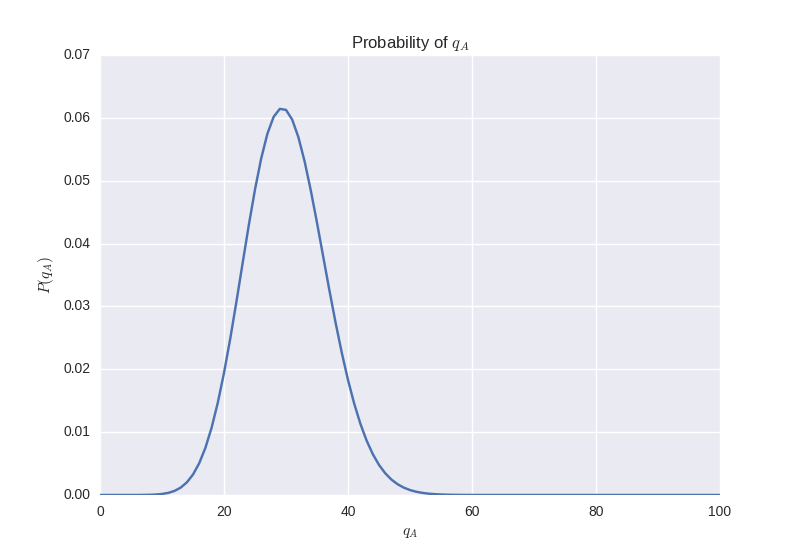
\includegraphics[scale=0.5]{gProb.png}
\caption{The probability of getting $q_A$ for $N_A = 30$, $N_B = 70$ and $q = 100$.}
\end{figure}

The program also shows us that the most likely macrostate is $q_A = 29$ with a probability of $0.0614$.

\subsection{h)}
We start by seeing that for \ref{eq:comb}, if $N>>1$ we get

\begin{equation}
\Omega(N,q) \approx \frac{(q+N)!}{q!N!}
\end{equation}


taking the logarithm of  we get

\begin{equation}
\ln \Omega(N,q) = \ln (q + N)! - \ln q! - \ln N!
\end{equation}

Then using Stirling's approximation $ \ln x! = x\ln x - x$:

\begin{equation}
\ln \Omega(N,q) = (q+N)\ln (q + N) - (q+N) - q\ln q + q - N\ln (N-1) +N
\end{equation}

\begin{equation}
= (q+N)\ln (q + N) - q\ln q - N\ln (N-1)
\end{equation}
	
We look at $\ln (q + N)$:

\begin{equation}
\ln (q + N) = \ln\left(q\left[1+\frac{N}{q}\right]\right) = \ln q + \ln\left(1+\frac{N}{q}\right)
\end{equation}

Since $N/q << 1$ we can use the Taylor expansion $\ln(1+x) \approx x$ of the last term and get

\begin{equation}
\ln (q + N) \approx \ln q + \frac{N}{q}
\end{equation}

We can now see that

\begin{equation}
\ln \Omega(N,q) \approx (q+N)\left(\ln q + \frac{N}{q}\right) - q\ln q - N\ln N = N\ln\frac{q}{N} + N + \frac{N^2}{q}
\end{equation}

But since $N/q << 1$ then $N^2/q$ become vanishingly small; for all intent and purposes zero:

\begin{equation}
\ln \Omega(N,q) \approx = N\ln\frac{q}{N} + N = N\left(\ln\frac{q}{N} + 1\right)
\end{equation}

\subsection{i)}

Entropy is given as

\begin{equation}
S \equiv k \ln \Omega(N,q)
\end{equation}\label{eq:entropy}

With $k$ being Boltzmann's constant. So we get the entropy for an Einstein crystal:

\begin{equation}
S = k\ln\left(\frac{(q+N-1)!}{q!(N-1)!}\right) \approx k N\left(\ln\frac{q}{N} + 1\right)
\end{equation}

\subsection{j)}
The temperature is given as

\begin{equation}
T = \left(\frac{\partial S}{\partial U}\right)^{-1} 
\end{equation}

$U$ is the energy and is proportional to $q$. So

\begin{equation}
U = mq \Rightarrow \frac{dU}{dq} = a \Rightarrow dU = adq
\end{equation}

So

\begin{equation}
T = \left(a\frac{\partial S}{\partial q}\right)^{-1} = \left(akN\frac{1}{N}\frac{1}{q/N}\right)^{-1} = \frac{q}{akN}
\end{equation}

\textbf{Commenter her!!}

\section{Part 2)}
\subsection{k)}

A particle can either have spin up or spin down. So for one particle we have two possible choices, and for the next particles there are two more microstates for each per state for the first particle. The next particle multiplies the number of microstates by 2, and so on. The number of possible microstates then becomes:

\begin{equation}
\Omega(N) = 2^N
\end{equation}

\subsection{i)}
The energy is given as

\begin{equation}
E = -S\mu B
\end{equation}

We want to find the total energy, where we have to sum over all the N particles:

\begin{equation}
E_{tot} = -\mu B\sum_{i = 0}^{N}S_i = -\mu B s = \mu B\frac{S_- - S_+}{2}
\end{equation}

\subsection{m)}

\textbf{GJØR!!!}

\subsection{n)}
We have N particles and what to see how many combinations that gives $S_+$. In other words, we have N and choose $S_+$, which means that the multiplicity is given as the binomial coefficient:

\begin{equation}
\Omega(N,S_+) = \binom{N}{S_+} = \frac{N!}{S_+!(N-S_+)!}
\end{equation}

Since we only have two possible spins the number of spin -1 has to be the total number of particles minus the number of spin +1, so $N-S_+ = S_-$, and

\begin{equation}
\Omega(N,S_+) = \frac{N!}{S_+!S_-!}
\end{equation}\label{ONS+}

\subsection{o)}

We now describe the system with the total spin $s = \sum_i S_i$. If the $s=0$ then there are the same number of +1 as -1, so $S_+ = S_- = N/2$. We also get from the exercise that $2s = S_+ - S_- = \Delta s$. If we have a non-zero spin we see that half of the difference in $S_+$ and $S_-$ has to come from $S_+$ and half from $S_-$. So

\begin{equation}
S_+ = \frac{N}{2} + \frac{\Delta s}{2} = \frac{N}{2} + s, \qquad S_- = \frac{N}{2} - \frac{\Delta s}{2} = \frac{N}{2} - s 
\end{equation}

We then see that we can rewrite \eqref{ONS+} as

\begin{equation}
\Omega(N,S_+) = \frac{N!}{(N/2 + s)!(N/2-s)!}
\end{equation}

\subsection{p)}


\end{document}




